\item
\mbox{}
\begin{center}
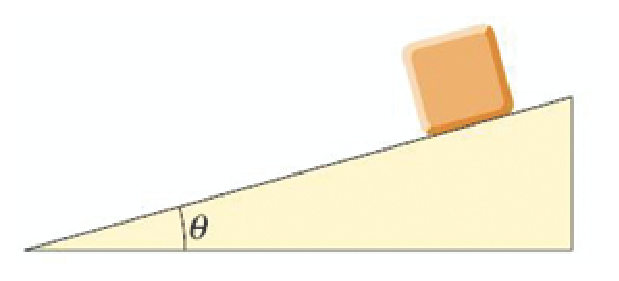
\includegraphics [scale=0.7]{./latex/eps/1_5_8_image_1.eps}
\end{center}
Gambar free-body balok diagram yang turun pada bidang miring dengan $\theta=15^{0}$, bila balok awalnya berada pada puncak dan panjang dari sisi miring 2 m, cari: \\
a. percepatan balok \\
b. kecepatan ketika mencapai meninggalkan bidang miring

\begin{description}
    \item[Solusi:]
        \mbox{}
\begin{center}
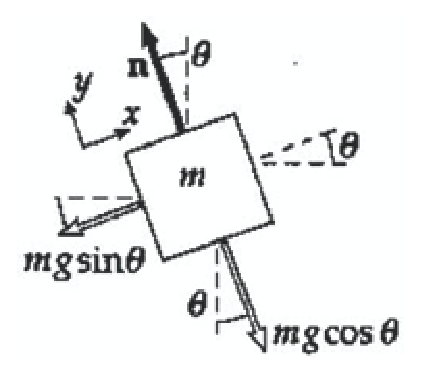
\includegraphics [scale=0.5]{./latex/eps/1_5_8_image_2.eps}
\end{center}
Gaya yang bekerja pada balok adalah gaya normal $n$ dan gaya gravitasi $mg$. Jika sumbu-x dipilih sejajar dengan bidang miring, maka free-body diagram dapat terlihat dari gambar. Dengan menggunakan hukum Newton II, didapat:
\begin{eqnarray*}
\Sigma F_{y}=0 \\
n-mg\cos\theta=0 \\
n=mg \cos\theta
\end{eqnarray*}
\begin{eqnarray*}
\Sigma F_{x}=0 \\
-mg\sin\theta=ma \\
a=-g \sin\theta
\end{eqnarray*}

a. Saat $\theta=15^{0}$ maka $a=-2.54$ $m/s^{2}$ \\
b. Karena benda mengalami percepatan konstan, maka berlaku
\begin{eqnarray*}
v_{f}^{2}-v_{i}^{2}=2as \\ 
\mbox{karena benda awalnya diam dan $s=2$m, maka} \\
v_{f}=\sqrt{2as}=\sqrt{2(-2.54)(-2.0)}= 3.18 \textrm{ m/s}
\end{eqnarray*} 
\end{description}
